\chapter{Interconnection Networks: Topology and Routing}\label{ch:interconnect}
\begin{center}\small\textit{How do thousands of cores, caches, and accelerators talk without drowning in wires?}\end{center}

\section{Why Interconnects Matter}
A single core is a fast worker on an isolated desk. A modern SoC or supercomputer is a
city: 64--1000 cores, GPU tiles, memory controllers, and I/O must all exchange data. The
streets and highways of this city are the \textbf{interconnection network} (IN). If the
network stalls, cores idle---Amdahl's serial fraction is not code but wire.

Early machines used a single shared \textbf{bus}: one set of wires, one transaction at a
time, snooped by all. Simple and coherent, but bandwidth is fixed and arbitration
serialises every miss. At 4 cores it suffices; at 64 it collapses. The bus is a one-lane
road into a metropolis.

We therefore replace the bus with scalable fabrics where many messages fly in parallel,
trading simple broadcast for richer topology, routing, and flow control. The design
space spans on-chip NoCs, off-chip supercomputer fabrics, and datacentre Clos
networks---same principles, different cost constraints.

\begin{definition}[Interconnection network metrics]
A topology is a graph $(V,E)$ where $V$ are nodes (cores/routers) and $E$ are links. Key
metrics: \emph{diameter} $D$ (max shortest path, worst latency), \emph{bisection
bandwidth} $B_{\text{bis}}$ (min links cut to halve the network, peak all-to-all
throughput), \emph{degree} $d$ (ports per router, cost), \emph{average distance}
$\bar{h}$ (mean hops), and \emph{cost} (routers + links + wiring area).
\end{definition}
Networks are judged by latency at low load, throughput at high load, and cost. A cheap
ring wins on cost but loses on diameter; an ideal crossbar wins on performance but loses
on cost ($O(N^2)$ switches). Real designs pick a point on this Pareto frontier.

\begin{center}
\begin{tikzpicture}[font=\scriptsize, scale=0.88]
% Bus
\node[draw, fill=blue!14, rounded corners, minimum width=5.2cm, minimum height=0.55cm] (bus) at (0,2.2) {\textbf{Bus}: shared medium --- one tx at a time};
\node[draw, fill=blue!8, minimum size=0.55cm] (n1) at (-1.8,3.0) {C}; \draw[thick, blue!60!black] (n1.south) -- (bus.north |- n1.south);
\node[draw, fill=blue!8, minimum size=0.55cm] (n2) at (-0.6,3.0) {C}; \draw[thick, blue!60!black] (n2.south) -- (bus.north |- n2.south);
\node[draw, fill=blue!8, minimum size=0.55cm] (n3) at (0.6,3.0) {C}; \draw[thick, blue!60!black] (n3.south) -- (bus.north |- n3.south);
\node[draw, fill=blue!8, minimum size=0.55cm] (n4) at (1.8,3.0) {C}; \draw[thick, blue!60!black] (n4.south) -- (bus.north |- n4.south);
\node[font=\tiny, text=red!70!black] at (0,1.65) {bandwidth $O(1)$, bottleneck};
% Crossbar
\node[draw, fill=green!14, minimum width=1.7cm, minimum height=1.7cm] (xb) at (-2.6,0) {Crossbar};
\foreach \y in {0.5,0,-0.5} {\fill[green!50!black] (-3.8,\y) circle (2pt); \draw[thick, green!50!black] (-3.8,\y) -- (-1.75,\y); \fill[orange!70!black] (-1.75,\y) circle (2pt);}
\node[font=\tiny, align=center] at (-2.6,-1.2) {non-blocking\\cost $O(N^2)$};
% Mesh fragment
\node[draw, fill=orange!18, circle, inner sep=1.8pt] (m11) at (1.2,0.6) {}; \node[draw, fill=orange!18, circle, inner sep=1.8pt] (m12) at (1.2,0) {}; \node[draw, fill=orange!18, circle, inner sep=1.8pt] (m13) at (1.2,-0.6) {};
\node[draw, fill=orange!18, circle, inner sep=1.8pt] (m21) at (2.2,0.6) {}; \node[draw, fill=orange!18, circle, inner sep=1.8pt] (m22) at (2.2,0) {}; \node[draw, fill=orange!18, circle, inner sep=1.8pt] (m23) at (2.2,-0.6) {};
\node[draw, fill=orange!18, circle, inner sep=1.8pt] (m31) at (3.2,0.6) {}; \node[draw, fill=orange!18, circle, inner sep=1.8pt] (m32) at (3.2,0) {}; \node[draw, fill=orange!18, circle, inner sep=1.8pt] (m33) at (3.2,-0.6) {};
\draw[thick, orange!60!black] (m11) -- (m21); \draw[thick, orange!60!black] (m21) -- (m31);
\draw[thick, orange!60!black] (m12) -- (m22); \draw[thick, orange!60!black] (m22) -- (m32);
\draw[thick, orange!60!black] (m13) -- (m23); \draw[thick, orange!60!black] (m23) -- (m33);
\draw[thick, orange!60!black] (m11) -- (m12); \draw[thick, orange!60!black] (m12) -- (m13);
\draw[thick, orange!60!black] (m21) -- (m22); \draw[thick, orange!60!black] (m22) -- (m23);
\draw[thick, orange!60!black] (m31) -- (m32); \draw[thick, orange!60!black] (m32) -- (m33);
\node[font=\tiny, align=center] at (2.2,-1.2) {$3\times3$ mesh, degree 4\\scalable $O(N)$};
\draw[{Stealth}-{Stealth}, thick, violet!70!black] (-0.6,0) -- (0.6,0) node[midway, above, font=\tiny, fill=white] {scale};
\end{tikzpicture}
\end{center}

\section{Topology Taxonomy}
\textbf{Direct networks}: each node has an integrated router (mesh, torus, hypercube).
\textbf{Indirect}: separate switch nodes connect terminals (crossbar, fat-tree, Clos).
Direct suits on-chip (NoC) where wiring is planar; indirect dominates off-chip
supercomputers where switch radix and cable length dominate.

\begin{itemize}[leftmargin=1.2em, itemsep=0.2em]
\item \textbf{Ring} ($N$ nodes, degree 2, $D=\lfloor N/2\rfloor$): cheapest, but diameter grows linearly. Bidirectional halves $D$.
\item \textbf{2-D mesh} ($k\times k$, $N=k^2$, degree $\le4$, $D=2(k-1)$, $B_{\text{bis}}=k$): layout-friendly, VLSI planar. Intel mesh NoC, Tilera.
\item \textbf{2-D torus}: mesh plus wrap-around links (degree 4, $D=k$, $B_{\text{bis}}=2k$): doubles bisection at cost of long wraps.
\item \textbf{Hypercube} ($N=2^d$, degree $d$, $D=d$, $B_{\text{bis}}=N/2$): logarithmic diameter, but degree grows with $N$---wiring explodes.
\item \textbf{Fat tree / Clos}: indirect, non-blocking with enough middle stages; $D=O(\log N)$, $B_{\text{bis}}=N/2$ at cost of many switches. Modern datacentres, NVLink, InfiniBand.
\end{itemize}
Meshes dominate chips because they map to 2-D silicon. At rack scale, fat-trees dominate
because bisection matters more than wire length. Understanding this split explains why
NoC papers show meshes and HPC papers show Clos.

\begin{center}
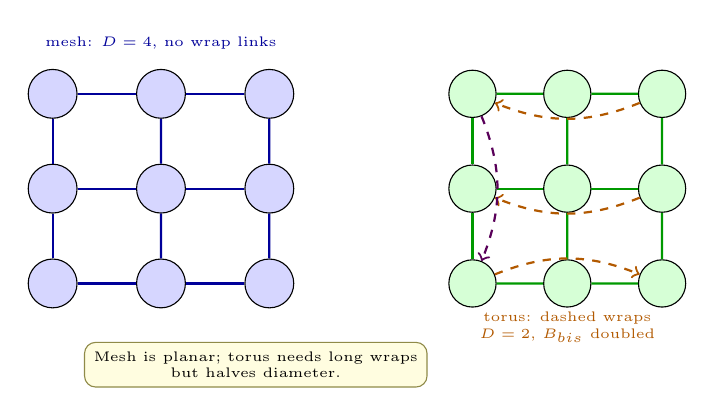
\begin{tikzpicture}[font=\scriptsize, scale=0.86]
% Mesh 3x3 left
\node[draw, fill=blue!16, circle, minimum size=0.62cm] (a11) at (0,1.4) {}; \node[draw, fill=blue!16, circle, minimum size=0.62cm] (a12) at (0,0) {}; \node[draw, fill=blue!16, circle, minimum size=0.62cm] (a13) at (0,-1.4) {};
\node[draw, fill=blue!16, circle, minimum size=0.62cm] (a21) at (1.6,1.4) {}; \node[draw, fill=blue!16, circle, minimum size=0.62cm] (a22) at (1.6,0) {}; \node[draw, fill=blue!16, circle, minimum size=0.62cm] (a23) at (1.6,-1.4) {};
\node[draw, fill=blue!16, circle, minimum size=0.62cm] (a31) at (3.2,1.4) {}; \node[draw, fill=blue!16, circle, minimum size=0.62cm] (a32) at (3.2,0) {}; \node[draw, fill=blue!16, circle, minimum size=0.62cm] (a33) at (3.2,-1.4) {};
\draw[thick, blue!60!black] (a11) -- (a21); \draw[thick, blue!60!black] (a21) -- (a31);
\draw[thick, blue!60!black] (a12) -- (a22); \draw[thick, blue!60!black] (a22) -- (a32);
\draw[thick, blue!60!black] (a13) -- (a23); \draw[thick, blue!60!black] (a23) -- (a33);
\draw[thick, blue!60!black] (a11) -- (a12); \draw[thick, blue!60!black] (a12) -- (a13);
\draw[thick, blue!60!black] (a21) -- (a22); \draw[thick, blue!60!black] (a22) -- (a23);
\draw[thick, blue!60!black] (a31) -- (a32); \draw[thick, blue!60!black] (a32) -- (a33);
\node[font=\tiny, text=blue!60!black] at (1.6,2.15) {mesh: $D=4$, no wrap links};
% Torus wraparound hint to the right
\begin{scope}[xshift=6.2cm]
\node[draw, fill=green!16, circle, minimum size=0.60cm] (b11) at (0,1.4) {}; \node[draw, fill=green!16, circle, minimum size=0.60cm] (b12) at (0,0) {}; \node[draw, fill=green!16, circle, minimum size=0.60cm] (b13) at (0,-1.4) {};
\node[draw, fill=green!16, circle, minimum size=0.60cm] (b21) at (1.4,1.4) {}; \node[draw, fill=green!16, circle, minimum size=0.60cm] (b22) at (1.4,0) {}; \node[draw, fill=green!16, circle, minimum size=0.60cm] (b23) at (1.4,-1.4) {};
\node[draw, fill=green!16, circle, minimum size=0.60cm] (b31) at (2.8,1.4) {}; \node[draw, fill=green!16, circle, minimum size=0.60cm] (b32) at (2.8,0) {}; \node[draw, fill=green!16, circle, minimum size=0.60cm] (b33) at (2.8,-1.4) {};
\draw[thick, green!60!black] (b11) -- (b21); \draw[thick, green!60!black] (b21) -- (b31);
\draw[thick, green!60!black] (b12) -- (b22); \draw[thick, green!60!black] (b22) -- (b32);
\draw[thick, green!60!black] (b13) -- (b23); \draw[thick, green!60!black] (b23) -- (b33);
\draw[thick, green!60!black] (b11) -- (b12); \draw[thick, green!60!black] (b12) -- (b13);
\draw[thick, green!60!black] (b21) -- (b22); \draw[thick, green!60!black] (b22) -- (b23);
\draw[thick, green!60!black] (b31) -- (b32); \draw[thick, green!60!black] (b32) -- (b33);
% wraparounds dashed
\draw[thick, orange!70!black, dashed, ->] (b31) to[bend left=22] (b11);
\draw[thick, orange!70!black, dashed, ->] (b32) to[bend left=22] (b12);
\draw[thick, orange!70!black, dashed, ->] (b13) to[bend left=22] (b33);
\draw[thick, violet!70!black, dashed, ->] (b11) to[bend left=22] (b13);
\node[font=\tiny, align=center, text=orange!70!black] at (1.4,-2.05) {torus: dashed wraps\\$D=2$, $B_{\text{bis}}$ doubled};
\end{scope}
\node[font=\tiny, fill=yellow!12, draw=yellow!50!black, rounded corners, align=center] at (3.0,-2.6) {Mesh is planar; torus needs long wraps\\but halves diameter.};
\end{tikzpicture}
\end{center}

\section{Routing: From Determinism to Adaptivity}
Routing picks the path a packet follows. Two independent decisions: \emph{which} path
and \emph{when} to wait for links.

\textbf{Dimension-order (DOR)} on a mesh: go first in $X$, then $Y$ (or $X$--$Y$).
Simple, deadlock-free by construction, but oblivious to congestion---a hot spot on the
$X$ row stalls all traffic. \textbf{Adaptive routing} senses congestion (queue depth,
credit count) and detours, improving throughput but risking deadlock, livelock (infinite
wandering), and out-of-order delivery.

\textbf{Deadlock}: cyclic buffer wait---four packets each holding one link waiting for
the next, none can advance. Classic on a $2\times2$ mesh with four packets circling
clockwise. Broken by ordering resources: DOR's $X\to Y$ order forbids the $Y\to X$ turn
that completes the cycle; or use \textbf{virtual channels (VCs)}---multiple logical
queues per physical link---to break cycles without restricting turns. VCs also cure
head-of-line blocking.

Flow control decides when flits move. \textbf{Store-and-forward}: whole packet buffered
per hop (high latency, large buffers). \textbf{Wormhole}: packet split into \emph{flits}
(flow-control units), flits pipeline across routers; header opens the path, body
follows; stalled header blocks body flits strung across routers (small buffers, low
latency, but head-of-line blocking). \textbf{Virtual-cut-through} is the middle ground:
forward as soon as next router has room for the whole packet.

\begin{lstlisting}[language=Python, caption={Dimension-order routing (X-then-Y) on a $k\times k$ mesh.}]
def dor_next_hop(src, dst, k):
    sx, sy = src % k, src // k
    dx, dy = dst % k, dst // k
    x, y = sx, sy
    path = [src]
    while x != dx:  # X dimension first
        x += 1 if dx > x else -1
        path.append(y * k + x)
    while y != dy:  # then Y dimension
        y += 1 if dy > y else -1
        path.append(y * k + x)
    return path  # e.g. dor_next_hop(0, 8, 3) -> [0,1,2,5,8]

# Adaptive variant: pick less-congested minimal direction
def adaptive_next(src, dst, congest):
    cand = minimal_directions(src, dst)  # up to 2 options
    return min(cand, key=lambda n: congest[n])
\end{lstlisting}

\begin{center}
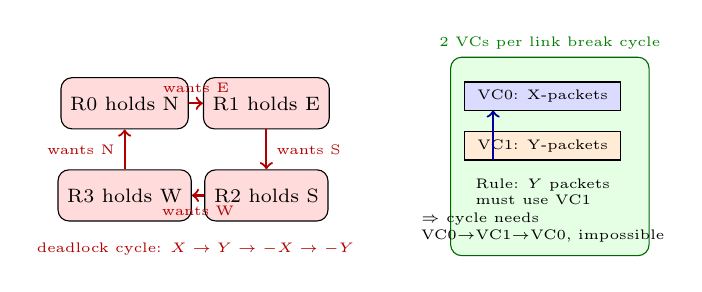
\begin{tikzpicture}[font=\scriptsize, scale=0.90]
% Deadlock cycle left
\node[draw, fill=red!14, minimum width=1.1cm, minimum height=0.65cm, rounded corners] (r0) at (0,1.0) {R0 holds N};
\node[draw, fill=red!14, minimum width=1.1cm, minimum height=0.65cm, rounded corners] (r1) at (2.0,1.0) {R1 holds E};
\node[draw, fill=red!14, minimum width=1.1cm, minimum height=0.65cm, rounded corners] (r2) at (2.0,-0.3) {R2 holds S};
\node[draw, fill=red!14, minimum width=1.1cm, minimum height=0.65cm, rounded corners] (r3) at (0,-0.3) {R3 holds W};
\draw[->, thick, red!70!black] (r0.east) -- (r1.west) node[midway, above, font=\tiny] {wants E};
\draw[->, thick, red!70!black] (r1.south) -- (r2.north) node[midway, right, font=\tiny] {wants S};
\draw[->, thick, red!70!black] (r2.west) -- (r3.east) node[midway, below, font=\tiny] {wants W};
\draw[->, thick, red!70!black] (r3.north) -- (r0.south) node[midway, left, font=\tiny] {wants N};
\node[font=\tiny, text=red!70!black, align=center] at (1.0,-1.05) {deadlock cycle: $X\to Y\to -X\to -Y$};
% VC breaking on right
\begin{scope}[xshift=4.8cm]
\draw[fill=green!10, draw=green!40!black, rounded corners] (-0.2,-1.15) rectangle (2.6,1.65);
\node[font=\tiny, text=green!50!black] at (1.2,1.85) {2 VCs per link break cycle};
\draw[fill=blue!14] (0,0.9) rectangle (2.2,1.3) node[midway, font=\tiny] {VC0: X-packets};
\draw[fill=orange!16] (0,0.2) rectangle (2.2,0.6) node[midway, font=\tiny] {VC1: Y-packets};
\node[font=\tiny, align=left] at (1.1,-0.25) {Rule: $Y$ packets\\must use VC1};
\node[font=\tiny, align=left] at (1.1,-0.75) {$\Rightarrow$ cycle needs\\VC0$\to$VC1$\to$VC0, impossible};
\draw[->, thick, blue!60!black] (0.4,0.2) -- (0.4,0.9);
\end{scope}
\end{tikzpicture}
\end{center}

\section{NoC Router and Flow Control}
A canonical NoC router has five ports (N/S/E/W + local), each with VC buffers, a
route-compute stage, VC allocator, switch allocator, and crossbar. Pipeline: RC $\to$ VA
$\to$ SA $\to$ ST (switch traversal) $\to$ LT (link traversal). Speculative allocation
collapses VA+SA for low load. Credit-based flow control keeps producer from overrunning
the next router: downstream advertises free flit slots; upstream sends only when credits
remain. This is lossless backpressure, essential for coherence messages that cannot be
dropped.

Power and area of the router matter: at 64 cores the NoC can be 15--25\% of chip area.
Optimisations include bufferless deflection routing (drop buffering, deflect on
conflict), concentrated meshes (4 cores share one router), and express virtual channels
(bypass intermediate routers).

\section{Performance: Latency, Throughput, Contention}
Zero-load latency $T_0 = H\cdot t_r + D/v + L/B$: hops $\times$ router delay plus wire
propagation plus serialisation ($L$ bytes at $B$ bytes/s). Under load, contention adds
queueing---modelled as $M/D/1$ per link, so latency rises steeply after $\sim$50\% of
saturation throughput.

Bisection bandwidth caps global throughput. For $k\times k$ mesh, $B_{\text{bis}}=k$
links $\times$ link BW. Doubling $k$ quadruples nodes but only doubles bisection---hence
meshes are bisection-limited at scale; torus and fat-trees trade cost for bisection.
Uniform random traffic saturates at $\approx B_{\text{bis}}/(\bar{h})$; adversarial
(transpose, hotspot) saturates far earlier, exposing the topology's weakness.

Wormhole's head-of-line blocking is eased by VCs: each VC has its own buffer, so a
stalled packet in VC0 does not block VC1 on the same wire. More VCs improve throughput
but add allocator complexity and power. Modern NoCs use 2--4 VCs, enough to separate
coherence classes (request/response) and break protocol deadlock.

\begin{lstlisting}[language=Python, caption={Wormhole flit pipeline: latency vs. store-and-forward.}]
def wormhole_latency(hops, t_r, t_w, flits, bw):
    # t_r: router pipeline per hop, t_w: wire, flits pipeline
    header = hops * (t_r + t_w)
    body   = (flits - 1) / bw  # flits stream behind header
    return header + body

def store_forward_latency(hops, pkt_bytes, bw, t_r):
    return hops * (pkt_bytes / bw + t_r)

print(wormhole_latency(4, 2, 1, 8, 1))   # ~12 + 7 = 19 cycles
print(store_forward_latency(4, 8, 1, 2)) # 4*(8+2)=40 cycles
# wormhole halves latency for multi-flit packets
\end{lstlisting}

\section{Exercises}
\begin{exercise}Bus vs.\ mesh: a 64-core chip runs coherence broadcasts each miss. Why does a bus saturate? Estimate bus transactions/s if each miss moves 64\,B at 20\,GB/s link BW, and compare to a $8\times8$ mesh with $B_{\text{bis}}=8$ links. When is a bus still preferable?\end{exercise}
\begin{exercise}For $k=8$ ($N=64$): compute diameter and bisection bandwidth for ring, $8\times8$ mesh, $8\times8$ torus, and $64$-node hypercube ($d=6$). Rank them and explain which metric matters for all-to-all vs.\ nearest-neighbour traffic.\end{exercise}
\begin{exercise}Show that $X$-$Y$ DOR on a mesh is deadlock-free by ordering resources. Construct a 4-node cycle that would deadlock with unrestricted minimal routing, and explain how 2 VCs (escape VC) break it without forbidding turns.\end{exercise}
\begin{exercise}Wormhole vs.\ store-and-forward: a 5-flit packet traverses 6 hops; $t_r=3$, $t_w=1$ cycle, link BW = 1 flit/cycle. Compute both latencies. If one link stalls for 10 cycles, how far does the wormhole packet ``stretch'' and which routers' buffers fill?\end{exercise}
\begin{exercise}Design a fat-tree for $N=16$ terminals with 4-port switches. How many switches per level? What bisection bandwidth does it provide vs.\ a $4\times4$ mesh? Why do datacentres prefer fat-trees despite higher switch count?\end{exercise}
